\documentclass{aastex61}
%Packages
\usepackage{graphicx}
\usepackage{soul, listings, xcolor}
\usepackage{amsmath}
\usepackage{url}
%Code environment details
\definecolor{dkgreen}{rgb}{0,0.6,0}
\definecolor{gray}{rgb}{0.5,0.5,0.5}
\definecolor{mauve}{rgb}{0.58,0,0.82}
\definecolor{grey}{gray}{0.95}
\lstset{frame=tb,
	escapeinside={(*@}{@*)},
	frame = single,
	aboveskip=3mm,
	belowskip=3mm,
	showstringspaces=false,
	columns=flexible,
	basicstyle={\small\ttfamily},
	numbers=none,
	numberstyle=\tiny\color{gray},
	keywordstyle=\color{blue},
	commentstyle=\color{dkgreen},
	stringstyle=\color{mauve},
	breaklines=true,
	breakatwhitespace=true,
}

%% The default is a single spaced, 10 point font, single spaced article.
%% There are 5 other style options available via an optional argument. They
%% can be envoked like this:
%%
%% \documentclass[argument]{aastex61}
%% 
%% where the arguement options are:
%%
%%  twocolumn   : two text columns, 10 point font, single spaced article.
%%                This is the most compact and represent the final published
%%                derived PDF copy of the accepted manuscript from the publisher
%%  manuscript  : one text column, 12 point font, double spaced article.
%%  preprint    : one text column, 12 point font, single spaced article.  
%%  preprint2   : two text columns, 12 point font, single spaced article.
%%  modern      : a stylish, single text column, 12 point font, article with
%% 		  wider left and right margins. This uses the Daniel
%% 		  Foreman-Mackey and David Hogg design.
%%
%% Note that you can submit to the AAS Journals in any of these 6 styles.
%%
%% There are other optional arguments one can envoke to allow other stylistic
%% actions. The available options are:
%%
%%  astrosymb    : Loads Astrosymb font and define \astrocommands. 
%%  tighten      : Makes baselineskip slightly smaller, only works with 
%%                 the twocolumn substyle.
%%  times        : uses times font instead of the default
%%  linenumbers  : turn on lineno package.
%%  trackchanges : required to see the revision mark up and print its output
%%  longauthor   : Do not use the more compressed footnote style (default) for 
%%                 the author/collaboration/affiliations. Instead print all
%%                 affiliation information after each name. Creates a much
%%                 long author list but may be desirable for short author papers
%%
%% these can be used in any combination, e.g.
%%
%% \documentclass[twocolumn,linenumbers,trackchanges]{aastex61}

%% AASTeX v6.* now includes \hyperref support. While we have built in specific
%% defaults into the classfile you can manually override them with the
%% \hypersetup command. For example,
%%
%%\hypersetup{linkcolor=red,citecolor=green,filecolor=cyan,urlcolor=magenta}
%%
%% will change the color of the internal links to red, the links to the
%% bibliography to green, the file links to cyan, and the external links to
%% magenta. Additional information on \hyperref options can be found here:
%% https://www.tug.org/applications/hyperref/manual.html#x1-40003





%% This is the end of the preamble.  Indicate the beginning of the
%% manuscript itself with \begin{document}.

\begin{document}

\title{Lab 3: Radio Interferometry \\ AST 443: Observational Techniques in Astronomy}

\date{Performed October 19, 2016, and Submitted \today}

\author{Joseph Monroy}

\author{Yogesh Mehta}


\begin{abstract}
The goal of this experiment was to measure the angular profile of the Sun through two methods: using a single dish radio antenna and using a radio interferometer. From these profiles and scans of an unresolved point source (geosynchronous satellite), we can determine the angular diameter of the Sun.

We obtained our data by using the Stony Brook Radio telescope, which is able to switch between single dish and interferometry mode. The data we obtained was did not allow us to get reasonable results, so we borrowed another lab groups data.

For the interferometric mode, we obtained an angular diameter of (insert here), and (insert here) for single dish mode. Comparing both to the literature value of the angular diameter of the Sun, 32', we can see that...
\end{abstract}

\section{Introduction} \label{sec:intro}
The field of radio astronomy has grown exponentially just in the past 80 years. Up until to this time, the radio spectrum has been out of reach due to the large telescope needed to measure the full wavelength. Through pioneers such as Karl Jansky and Grote Reber, scientists began to see the true power of the radio spectrum. 

For many years astronomers kept improving the technology; however, they were always limited by the size of the telescope since you need a large diameter to resolve the huge radio wavelengths Also, it took a long time and always cost a lot to build these near football size telescope dishes. A breakthrough happened in the mid 1940's when astronomers started to apply the properties of interferometry to radio telescopes. Instead of having one huge telescope dish, you could use many, smaller telescopes over a large baseline to have the same effect. Now that the resolution simply depends on the baseline (the length of the array of telescopes), we can have radio interferometers that span many kilometers.

This is the technique we are trying to show in our experiment, and how it results in far better data then if you simply have one telescope. 

\section{Observations}
We first took our data on October 19th 2016 using the Stony Brook University Radio Telescope. This telescope was specifically designed and built by Professor Jin Koda as a cheap, simple alternative for those wanting to conduct amateur radio observations. It consists of a single 1 meter diameter satellite dish attached to an azimuthal and altitude drive. Placed below this dish is a long ladder, on which we place the two flat mirrors on both sides of the dish in interferometric mode. Also directly behind the dish are receiver mirrors that reflect the incoming radio waves into the feed horn of the satellite. When we are in single dish mode, we can simply remove since they are not needed. An image of this setup is shown below:
\begin{figure}[hbt!]
	\centering
	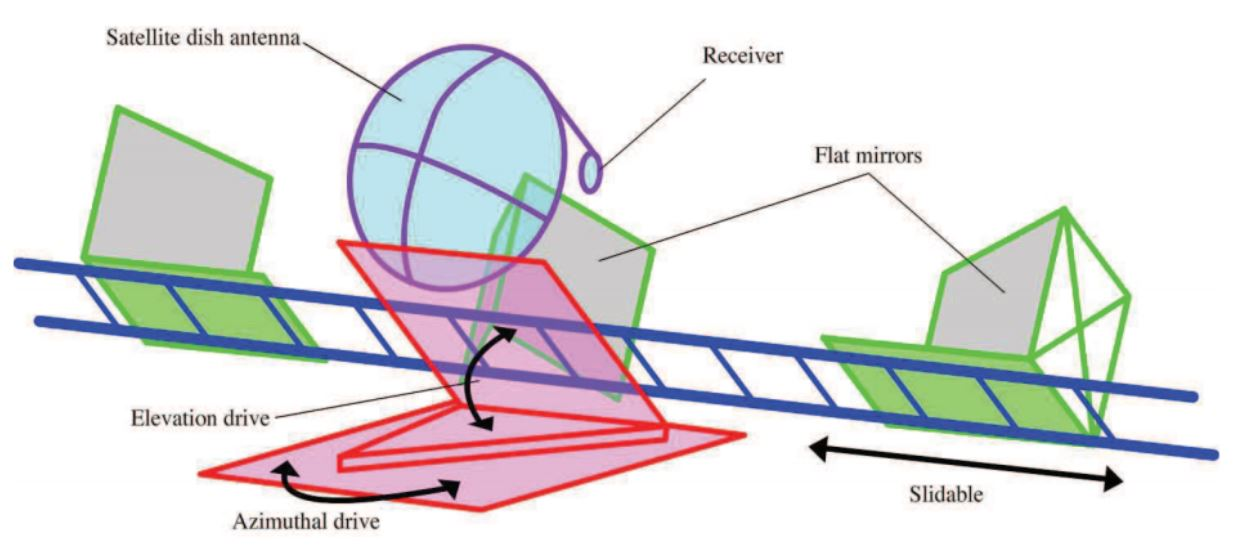
\includegraphics[scale = .45]{tourels.jpg}
	\caption{Diagram of the Stony Brook Radio Telescope in interferometry mode}
	\label{fig: refcurve1}
\end{figure}

We choose to put the telescope just outside the Physics building on Stony Brook University's West Campus, because it was a good place where the Sun would be visible for most of the day. The weather that day was mostly cloudy, with there being times we could not even find the Sun. Once we set up and put together the telescope, we began to calibrate the pointing of it in both single dish and interferometry mode. This was done by adjusting the azimuthal and altitude angles of the telescope such that we were just pointing next to the Sun. We then took an azimuthal scan of the Sun and noticed how many volts we were getting on the voltmeter. Depending on the mode we were in, we were supposed to see a specific pattern as a we scanned across the Sun. If we didn't get the expected result we went inside the voltmeter as switched out the attenuator for another one. We continued this until we got expected pattern, and therefore calibrated the telescope. 

Now we were able to start collecting our science data. For each time we scanned across an object, we made sure to right down the current time, the azimuth and altitude of the object, and start end azimuthal angles we scanned across. Also, we made sure to keep the slew rate of the dish as constant throughout the experiment. We started by taking data in single dish mode, taking two scans of the Sun. Next we choose a reference geosynchronous satellite that was far in position from the Sun. It took a while until we found a suitable one, but we eventually found one and took a scan of it two times. Now we switched the telescope into interferometry mode by flipping the dish around and placing all the mirrors back on the ladder. We choose to scan across the Sun in this mode five separate times, once for each different, $B$, baseline. The baseline could be read off by the ruler attached to the ladder. After scanning the Sun in all the baselines, we went back to our reference satellite and took scans of it for the same baselines used for the Sun.  

\section{Data Reduction}
The data we recorded was taken from a laptop in the form of .CMBL files. These file types are used to view data in Logger Pro, however we are more interested in .CSV files. This file type basically separates data in columns spaced by columns. We converted all our data into this file type by using an online converter. The computer recorded our data as voltage with respect to time, so we are going to have to convert the time to azimuthal angle. This can be done by knowing the azimuthal angles in the beginning and end of the scans. And since we have a constant slew rate, we therefore can deduce the angle at each recorded time.

For the interferometric data, we first need to get the visibility $V_{0}$ at each baseline measurement. This is given by:
\begin{equation}
	V_{0}(B_{\lambda}) = \frac{P_{max}-P_{min}}{P_{max}+P_{min}}
\end{equation}
Where $P_{max}$ and $P_{min}$ represents the maximum amplitude fringe and successive minimum respectively. An example of what this should look like is shown below:
\begin{figure}[hbt!]
	\centering
	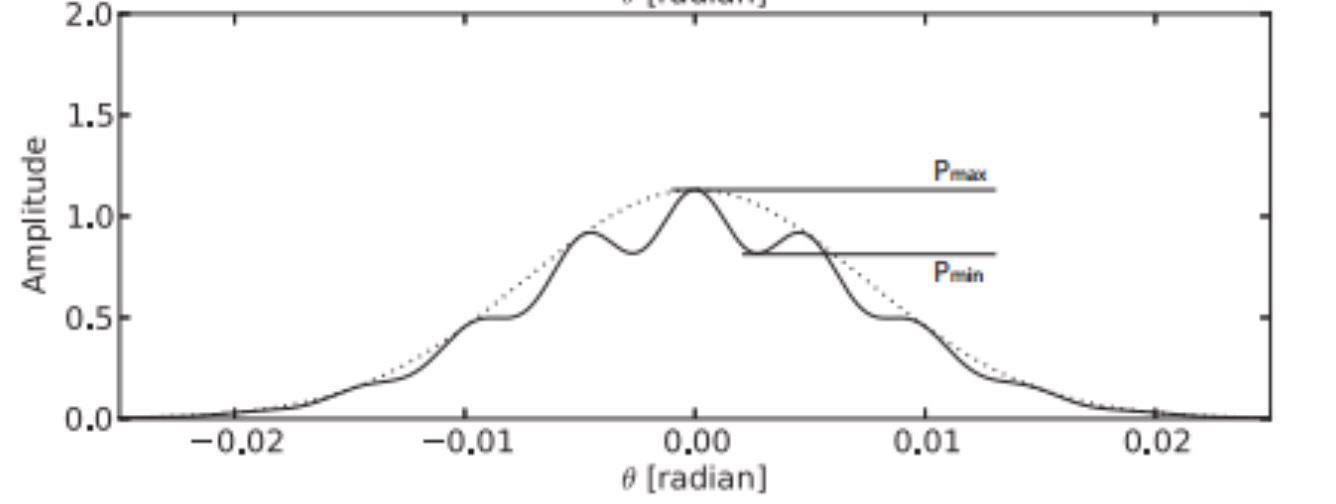
\includegraphics[scale = .45]{aaaa.jpg}
	\caption{This plot is taken from Professor Jin Koda's Journal article on this radio telescope}
	\label{fig: refcurve1}
\end{figure}
The independent variable $B_{\lambda}$ represents the baseline expressed in multiples of the radio wavelength. In our case, the radio wavelength we used was around 2.6 cm.. We can get this variable directly from our measurements from looking directly at our fringe profile for the satellite. Based on the angular length of a fringe pattern, we can directly get the baseline in multiples of wavelength. This is shown below:
\begin{equation}
	\delta\theta = \frac{\lambda}{B} = \frac{1}{B_{\lambda}}
\end{equation}
Where $\delta\lambda$ is taken from the plot:
\begin{figure}[hbt!]
	\centering
	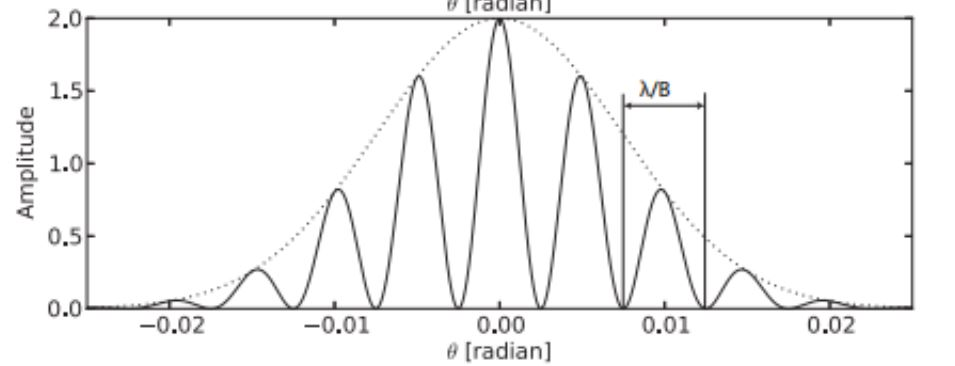
\includegraphics[scale = .45]{assssssssssssss.jpg}
	\caption{This is also taken from Professor Jin Koda's Journal article.}
	\label{fig: refcurve1}
\end{figure}
Once we have the visibility for each baseline, we can plot them against each other. From this plot we can deduce the diameter of the Sun through curve fitting.

The single dish data is a lot easier to analyze. All we need to do is to convert the time to azimuthal angle by the method stated before. We can plot the Sun and satellite data on the same curve to compare the angular profiles.

Unfortunately, we were unable to obtain any data we could reduce to get valuable data. Figures of our analyzed data in both modes can be seen in Figures 4 and 5.
\begin{figure}[hbt!]
	\centering
	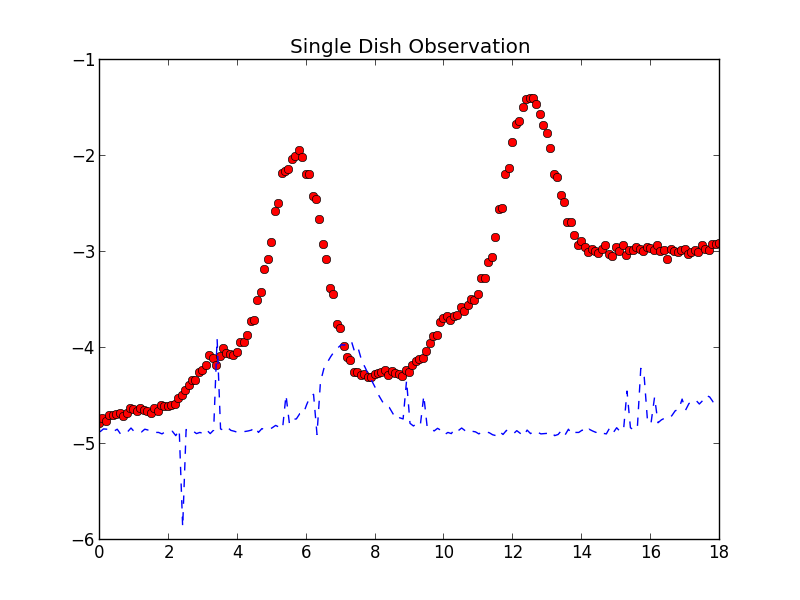
\includegraphics[scale = .45]{qqq.png}
	\caption{Plot of our Sun is the blue dashed line, while the satellite is in the red dots.}
	\label{fig: refcurve1}
\end{figure}
\begin{figure}[hbt!]
	\centering
	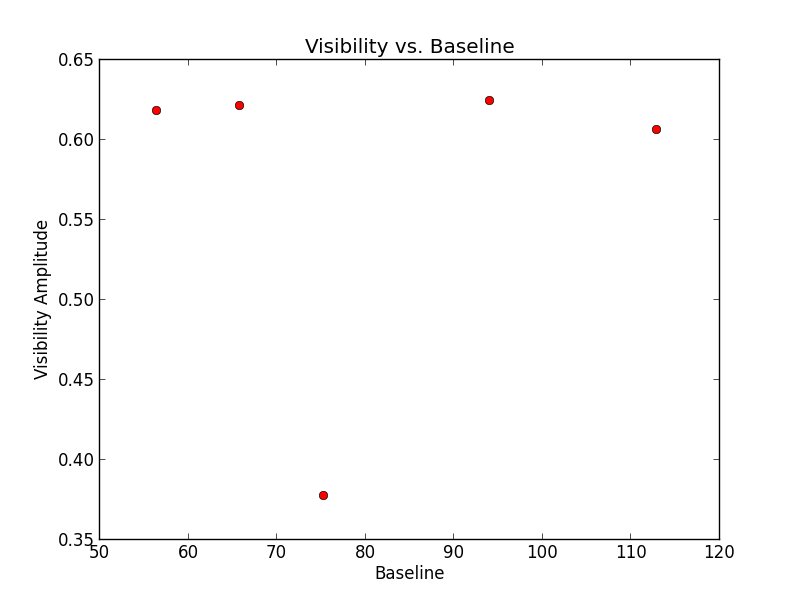
\includegraphics[scale = .45]{figure_1.png}
	\caption{Plot of our reduced interferometry mode data}
	\label{fig: refcurve1}
\end{figure}

As you can see, we can't obtain any reasonable results from this. It appears that when we took the single dish data for the satellite, we actually scanned across two satellites. The visibility vs. baseline plot does not resemble a sinc function by any means as well. So as a result, we decided to use the data taken by another lab group. Analyzing their data using the same methods stated earlier, we get the following figures:
\section{Data Analysis and Results}
Now that we have the plot of visibility vs. baseline, we can fit the plot to a sinc curve and get the diameter from the parameters. In theory, this plot should resemble a sinc function given by:
\begin{equation}
\sin\textit{c}(x) = \frac{\sin(\pi x)}{\pi x}
\end{equation}
Assuming the Sun to be a one dimensional disk, we can get the relation:
\begin{equation}
V_{0}(B_{\lambda}) = \frac{\sin(\pi B_{\lambda} \alpha)}{\pi B_{\lambda}}
\end{equation}
So if we fit the points to a sinc function, the parameter $\alpha$ should give us the angular diameter of the Sun
\section{Discussion}

\section{Conclusion }



\begin{thebibliography}{9}	
	
\end{thebibliography}

\appendix

\end{document}